\clearpage
\subsubsection{Continue} % (fold)
\label{sub:continue}

The continue statement is used to jump to the condition of the current loop. This is useful for skipping the processing of the current loop, but to allow the loop to continue for the next cycle.

\begin{figure}[h]
   \centering
   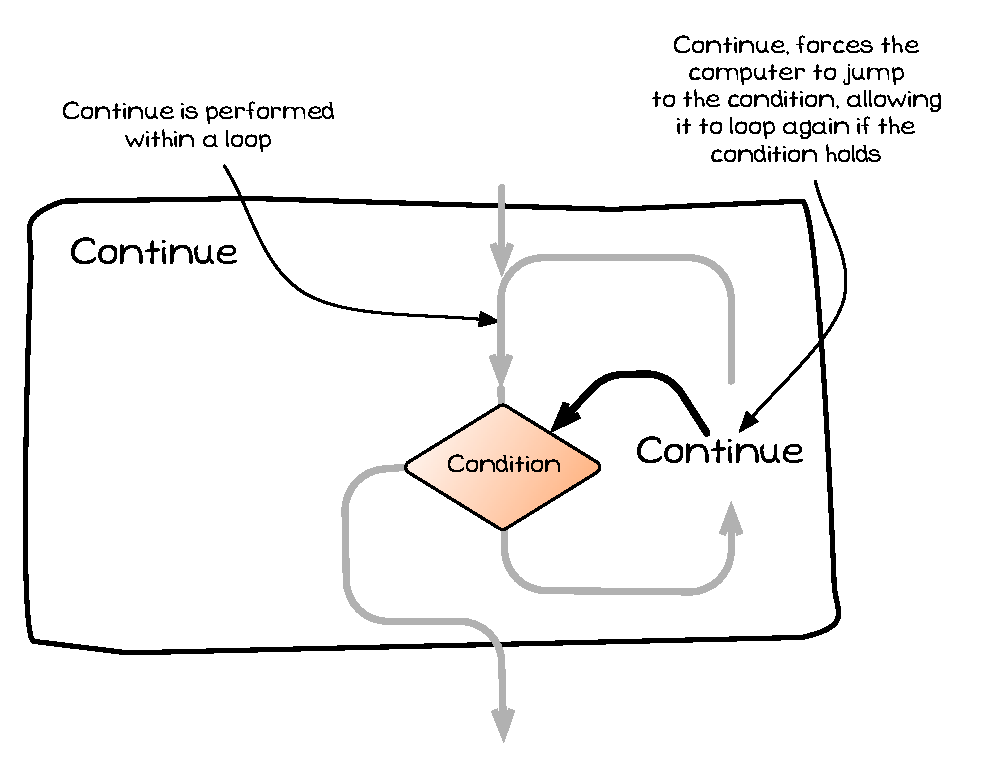
\includegraphics[width=\textwidth]{./topics/control-flow/diagrams/Continue} 
   \caption{The continue Statement allows you to jump to the condition, skipping the remainder of the code in the loop but allowing the loop to continue}
   \label{fig:continue}
\end{figure}

\mynote{
\begin{itemize}
  \item The continue statement is an \textbf{action}, allowing you to jump to the condition of the current loop.
  \item The continue statement should be coded within an \nameref{sub:branching} statement that checks if the loop should skip processing of the current cycle.
\end{itemize}
}


% subsection break (end)